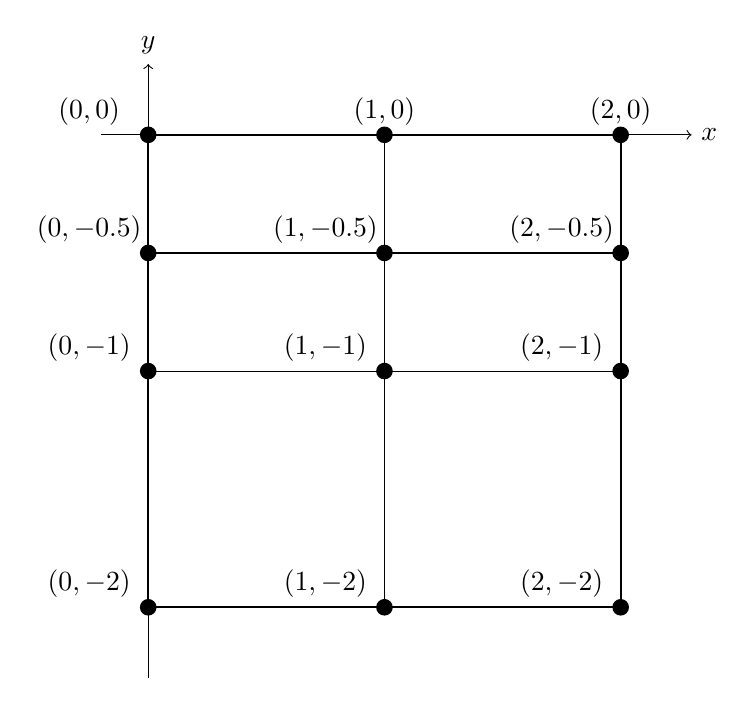
\begin{tikzpicture}[scale=3]

% Ejes
\draw[->] (-0.2,0) -- (2.3,0) node[right] {$x$};
\draw[->] (0,-2.3) -- (0,0.3) node[above] {$y$};

% Rectángulo A
\draw[thick] (0,-2) rectangle (2,0);

% Líneas de la partición en x
\draw (1,-2) -- (1,0);

% Líneas de la partición en y
\draw (0,-1) -- (2,-1);
\draw (0,-0.5) -- (2,-0.5);

% Puntos de la partición
\foreach \x in {0,1,2} {
    \foreach \y in {-2,-1,-0.5,0} {
        \fill (\x,\y) circle (0.5pt);
    }
}

% Puntos
\fill (0,0) circle (1pt);
  \node[above] at (-0.25,0) {$(0,0)$};

\fill (1,0) circle (1pt);
  \node[above] at (1,0) {$(1,0)$};

\fill (2,0) circle (1pt);
  \node[above] at (2,0) {$(2,0)$};

\fill (0,-0.5) circle (1pt);
  \node[above] at (-0.25,-0.5) {$(0,-0.5)$};

\fill (1,-0.5) circle (1pt);
  \node[above] at (0.75,-0.5) {$(1,-0.5)$};

\fill (2,-0.5) circle (1pt);
  \node[above] at (1.75,-0.5) {$(2,-0.5)$};

\fill (0,-1) circle (1pt);
  \node[above] at (-0.25,-1) {$(0,-1)$};

\fill (1,-1) circle (1pt);
  \node[above] at (0.75,-1) {$(1,-1)$};

\fill (2,-1) circle (1pt);
  \node[above] at (1.75,-1) {$(2,-1)$};

\fill (0,-2) circle (1pt);
  \node[above] at (-0.25,-2) {$(0,-2)$};

\fill (1,-2) circle (1pt);
  \node[above] at (0.75,-2) {$(1,-2)$};

\fill (2,-2) circle (1pt);
  \node[above] at (1.75,-2) {$(2,-2)$};

\end{tikzpicture}
